\documentclass{article}

% Language setting
% Replace `english' with e.g. `spanish' to change the document language
\usepackage[english]{babel}

% Set page size and margins
% Replace `letterpaper' with `a4paper' for UK/EU standard size
\usepackage[letterpaper,top=2cm,bottom=2cm,left=3cm,right=3cm,marginparwidth=1.75cm]{geometry}

% Useful packages
\usepackage{amsmath}
\usepackage{graphicx}
\usepackage[colorlinks=true, allcolors=blue]{hyperref}

\title{Rapport}
\author{Jean-emmanuel Chouinard (20246807), Timothe Payette (20239892)}
\date{12 juin 2023}

\begin{document}
\maketitle

\section{Auto-évaluation}

Notre programme fonctionne comme prévu. Il respecte les consignes et le format des sorties demandé. Par contre, la règle des longitudes et latitudes n'est pas respectée. Ceci est correct puisque le démonstrateur en tiendra compte lors de sa correction :) .

\section{Analyse de la complexité temporelle (pire cas) théorique en notation grand O}

\begin{figure}[htp]
\centering
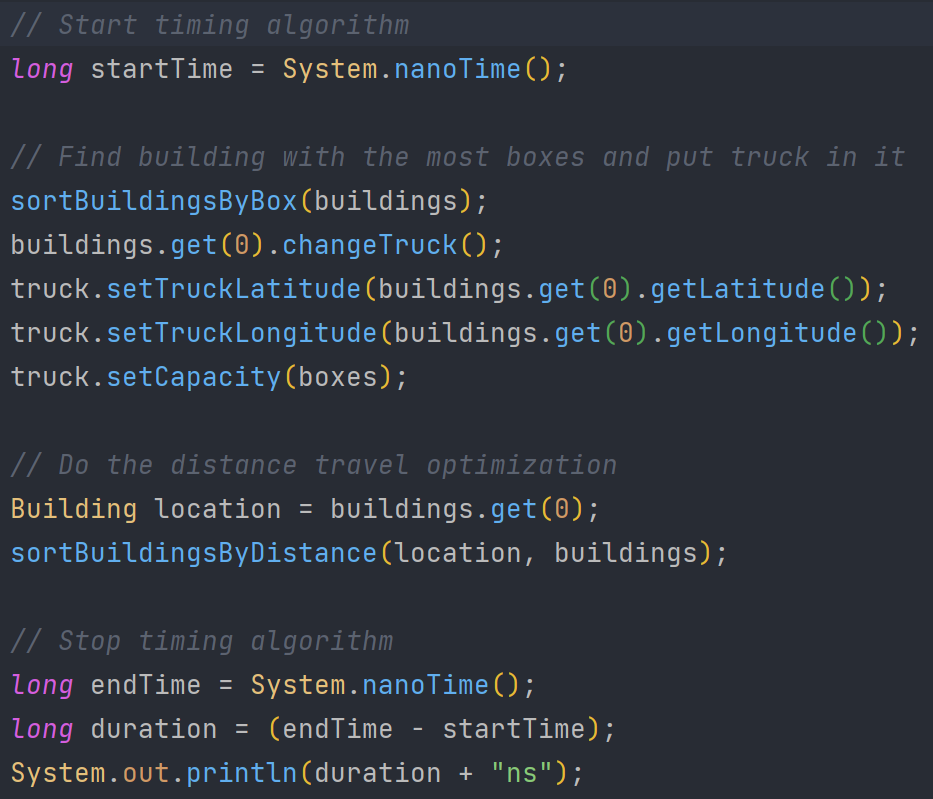
\includegraphics[width=0.5\textwidth]{algo.png}
\end{figure}

Notre programme peut être divisé en deux principales section. La première section tri la liste d'entrepôt (ici nommé building) en fonction du nombre de boites qu'il contient. De cette manière, il est assuré que le premier élément de la liste est celui avec le plus de boite. Voici la fonction $sortBuildingsByBox$.

\begin{figure}[htp]
\centering
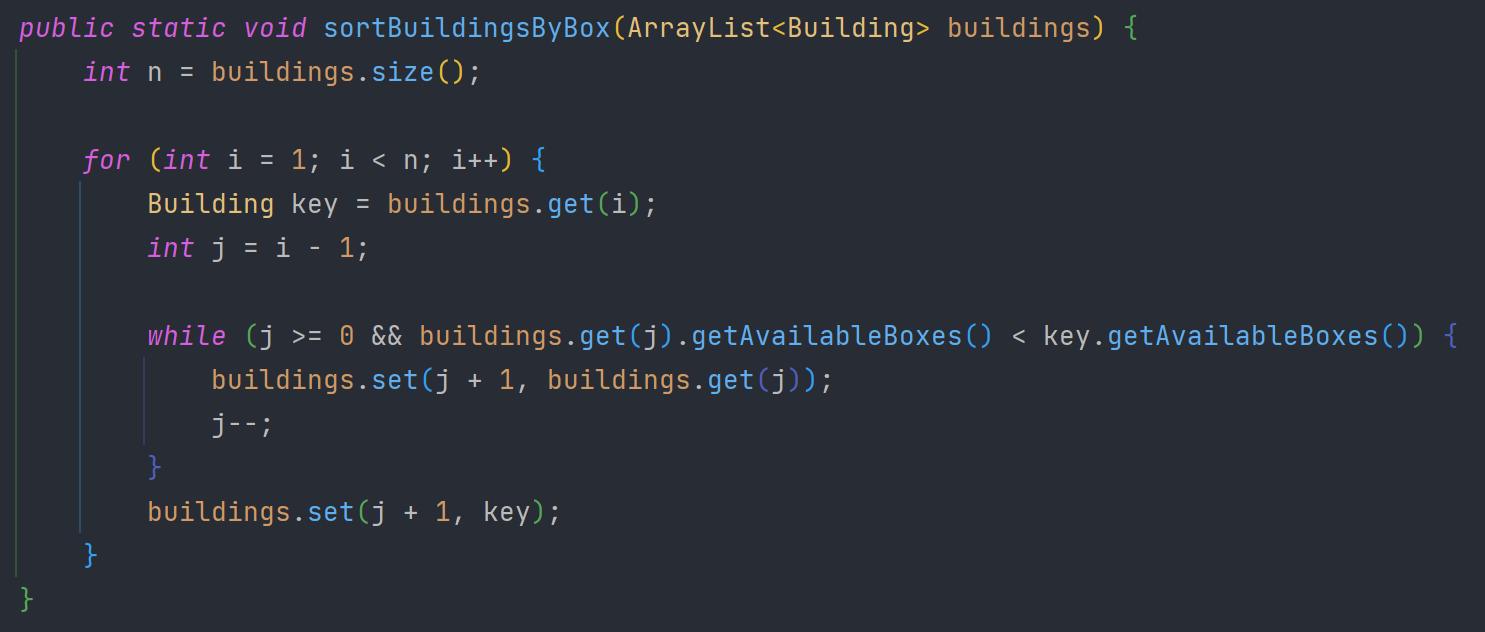
\includegraphics[width=0.5\textwidth]{sortBuilding.png}
\end{figure}

Dans cette fonction de tri, nous passons à travers la liste de buildings deux fois dans le pire des cas (soit que la liste est classée en ordre décroissante), ce qui rend notre algorithme de complexité $O(n^2)$ où n est le nombre de buildings dans la liste.
\\ \\
Observons la deuxième partie de l'algorithme où la liste est triée en fonction de la distance entre le premier élément de la liste et les autres.

\begin{figure}[htp]
\centering
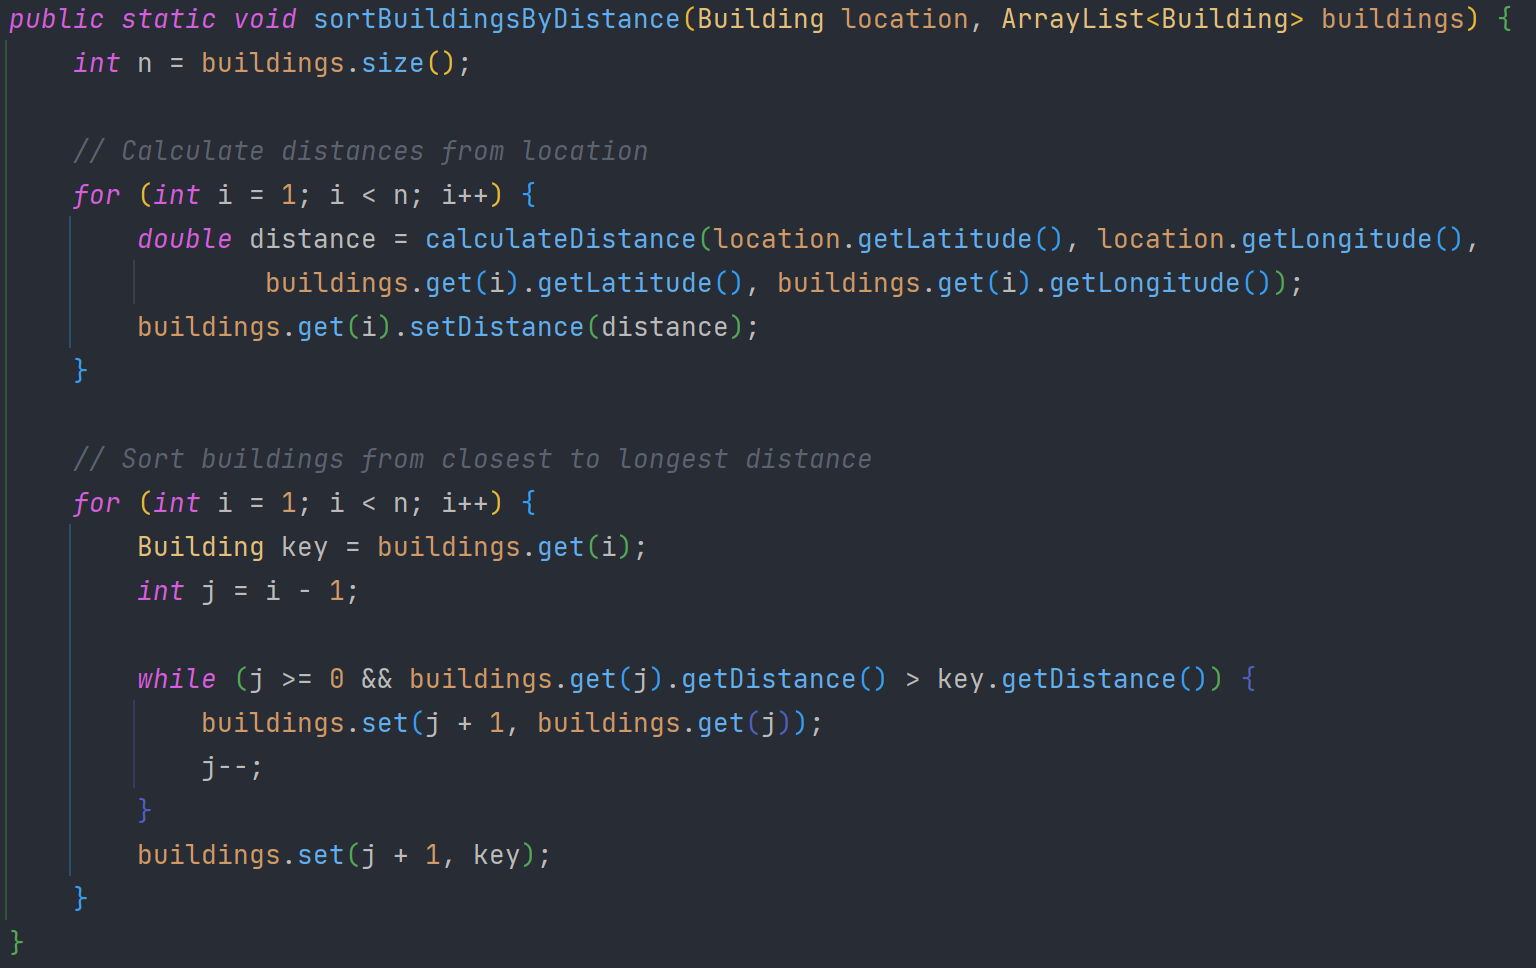
\includegraphics[width=0.5\textwidth]{sortDistance.png}
\end{figure}

Dans cette fonction de tri, nous passons deux fois à travers la liste dans le pire des cas. Comme celle de $sortBuildingsByBox$, la complexité est de $O(n^2)$. De plus, le calcul des distances entre les buildings et le camion a une complexité de $O(n)$. Finalement, cette fonction a une complexité de $O(n^2) + O(n) = O(n^2)$.
\\ \\
En bout de ligne, notre algorithme de tri a une complexité de $O(n^2) + O(n^2) = O(n^2)$.

\section{Analyse de la complexité temporelle empirique}

\begin{figure}[htp]
\centering
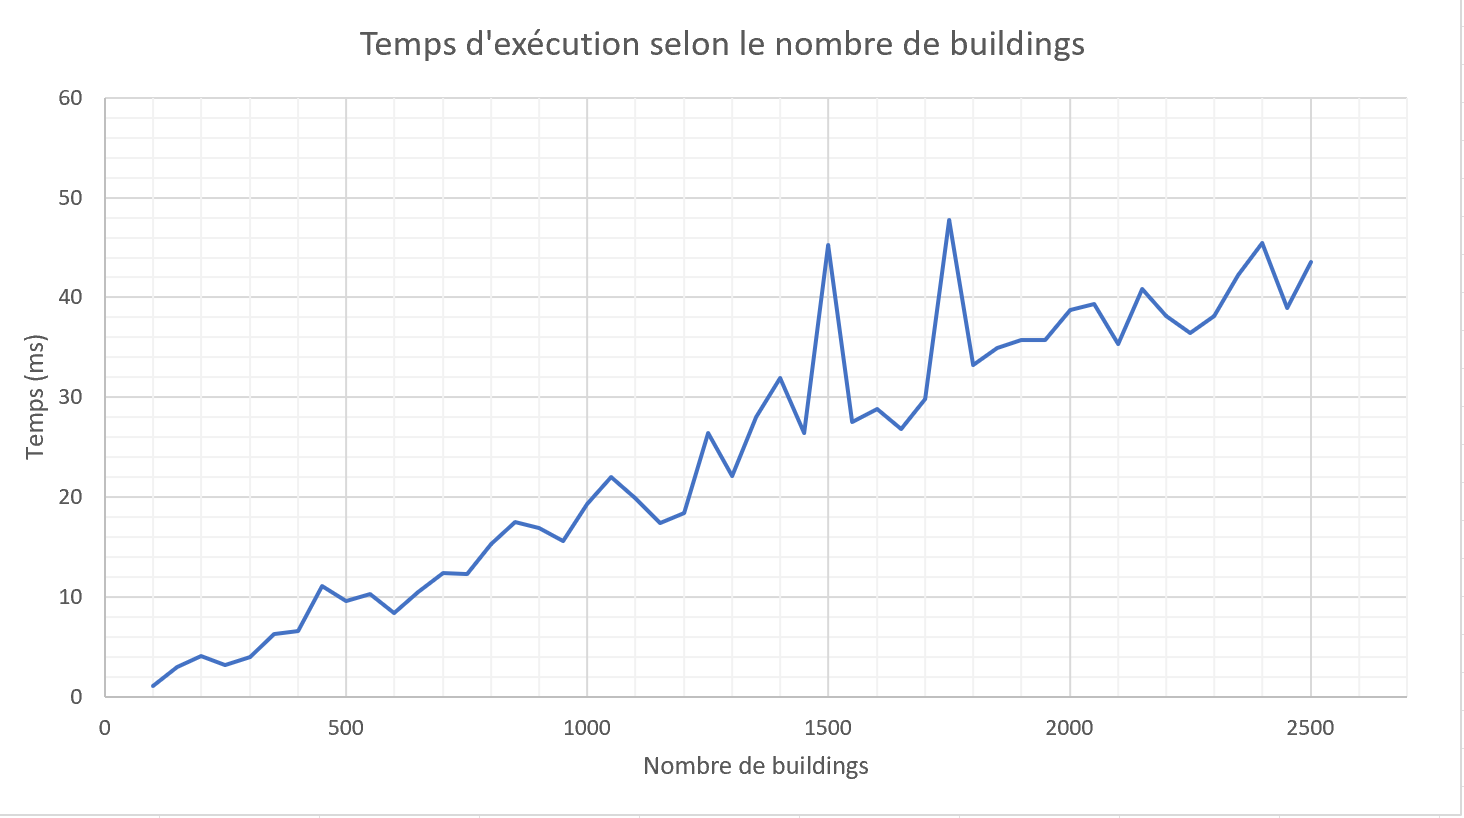
\includegraphics[width=0.5\textwidth]{analyse.png}
\end{figure}

Les données utilisées (n) pour ce graphique vont de 100 à 2500 par bond de 50.

\end{document}